\documentclass{article}
\usepackage{tabularx}
\usepackage{graphicx}
\usepackage{dirtytalk}
\usepackage{pgfplotstable} 
\usepackage{pgfplots}
\usepackage{datatool}
\usepackage{siunitx}
\usepackage[hyphens]{url}
\usepackage{hyperref}
\usepackage{graphicx}
\usepackage{microtype}
\usepackage{float}
\usepackage[style=ieee]{biblatex}
\usepackage{listings}
\usepackage{xcolor}
\usepackage[normalem]{ulem}
\usepackage{dirtytalk}

\definecolor{mygreen}{rgb}{0,0.6,0}
\definecolor{mygray}{rgb}{0.5,0.5,0.5}
\definecolor{mymauve}{rgb}{0.58,0,0.82}

\lstset{
    language=Java,                % Set language to Java
    basicstyle=\ttfamily\footnotesize, % Set font style and size
    keywordstyle=\color{blue},    % Set color for keywords
    stringstyle=\color{mymauve},  % Set color for strings
    commentstyle=\color{mygreen}, % Set color for comments
    numbers=left,                 % Line numbers on the left
    numberstyle=\tiny\color{mygray}, % Style for line numbers
    stepnumber=1,                 % Line number step size
    numbersep=10pt,               % Line number separation
    backgroundcolor=\color{white},% Background color
    showspaces=false,             % Do not show spaces
    showstringspaces=false,       % Do not underline spaces in strings
    showtabs=false,               % Do not show tabs
    frame=single,                 % Draw a frame around the code
    tabsize=4,                    % Set tab size
    captionpos=b,                 % Caption position (bottom)
    breaklines=true,              % Allow line breaking
    breakatwhitespace=false,      % Line breaks only at whitespace
    title=\lstname                % Show the filename of the code
}

\lstdefinestyle{bash}{
    language=bash,                % Set language to Bash
    basicstyle=\ttfamily\footnotesize, % Set font style and size
    keywordstyle=\color{blue},    % Set color for keywords
    stringstyle=\color{mymauve},  % Set color for strings
    commentstyle=\color{mygreen}, % Set color for comments
    numbers=left,                 % Line numbers on the left
    numberstyle=\tiny\color{mygray}, % Style for line numbers
    stepnumber=1,                 % Line number step size
    numbersep=10pt,               % Line number separation
    backgroundcolor=\color{white},% Background color
    showspaces=false,             % Do not show spaces
    showstringspaces=false,       % Do not underline spaces in strings
    showtabs=false,               % Do not show tabs
    frame=single,                 % Draw a frame around the code
    tabsize=4,                    % Set tab size
    captionpos=b,                 % Caption position (bottom)
    breaklines=true,              % Allow line breaking
    breakatwhitespace=false,      % Line breaks only at whitespace
    title=\lstname                % Show the filename of the code
}

\addbibresource{main.bib}

\hypersetup{
    colorlinks=true,
    linkcolor=blue,
    filecolor=blue,      
    urlcolor=blue,
    citecolor=blue,
}

\pgfplotsset{compat=1.18}

\title{\textbf{Lab 2 - Parallel Sorting Algorithms\\Parallel and Distributed Computing\\DD2443 - Pardis24}}
\author{Names:\\Casper Kristiansson\\Nicole Wijkman\\\\Group 14}
\date{\today}

\begin{document}

\setlength\parindent{0pt}
\setlength{\parskip}{\bigskipamount}

\maketitle

\newpage
\section{Sequential Sort}

\subsection{Program Explanation}
\textbf{Source files:}

- `SequentialSort.java`

\subsubsection{Explanation}
For the sequential sorting algorithm, we chose to implement quicksort to sort integer arrays. The \texttt{sort()} method begins by calling the \texttt{quickSort()} function, which then recursively partitions the array and sorts each partition. The partitioning function selects the last element as the pivot and rearranges the array such that all elements smaller than the pivot are on the left, and larger elements are on the right. This process repeats for each subarray until the entire array is sorted. Since this is a sequential sort, only a single thread is used for execution.

\subsubsection{Discussion}
The sequential quicksort implementation performs as expected with consistent results. Since it operates with a single thread, there is no overhead related to thread management or synchronization, which can benefit smaller arrays. However, the performance is limited by the lack of parallelism, and it scales poorly with larger data sets or higher computational demands. In our test with an array size of 1000, the average execution time was approximately 51,316 nanoseconds, demonstrating that sequential sorting is efficient for small arrays but becomes a bottleneck for larger ones.

\newpage
\section{Amdahl’s Law and Speedup}

\subsection{Formulation of Amdahl’s Law}
Amdahl's Law estimates the potential speedup of a parallel algorithm by dividing the task into a parallelizable portion, \(p\), and a sequential portion, \(1 - p\). In quicksort, parallelization helps up to a point, but as thread count increases, the benefit diminishes due to overhead and small sub-arrays that gain little from parallelization.

To account for this, we modified Amdahl’s Law with a quadratic decay for thread effectiveness:

\[
S = \frac{1}{(1 - p) + \frac{p}{T^2}}
\]

Where:
 \begin{enumerate}
     \item[-] \( p \) is the parallelizable portion.
     \item[-] \( T \) is the number of threads.
     \item[-] \( T^2 \) reflects the faster diminishing returns as more threads are added, capturing quicksort’s behavior.
 \end{enumerate}

This formulation better models quicksort's performance, where beyond 4 to 8 threads, adding more threads yields limited gains due to overhead.

\subsection{Results and Plot}
The plot below shows the speedup using the modified Amdahl’s Law for 2, 4, 8, and 16 threads, with different values of \(p\) (0.2, 0.4, 0.6, 0.8). The quadratic term \(T^2\) causes the speedup to level off more quickly, reflecting how overhead reduces the benefit of adding more threads in parallelized quicksort.

\begin{figure}[H]
    \centering
    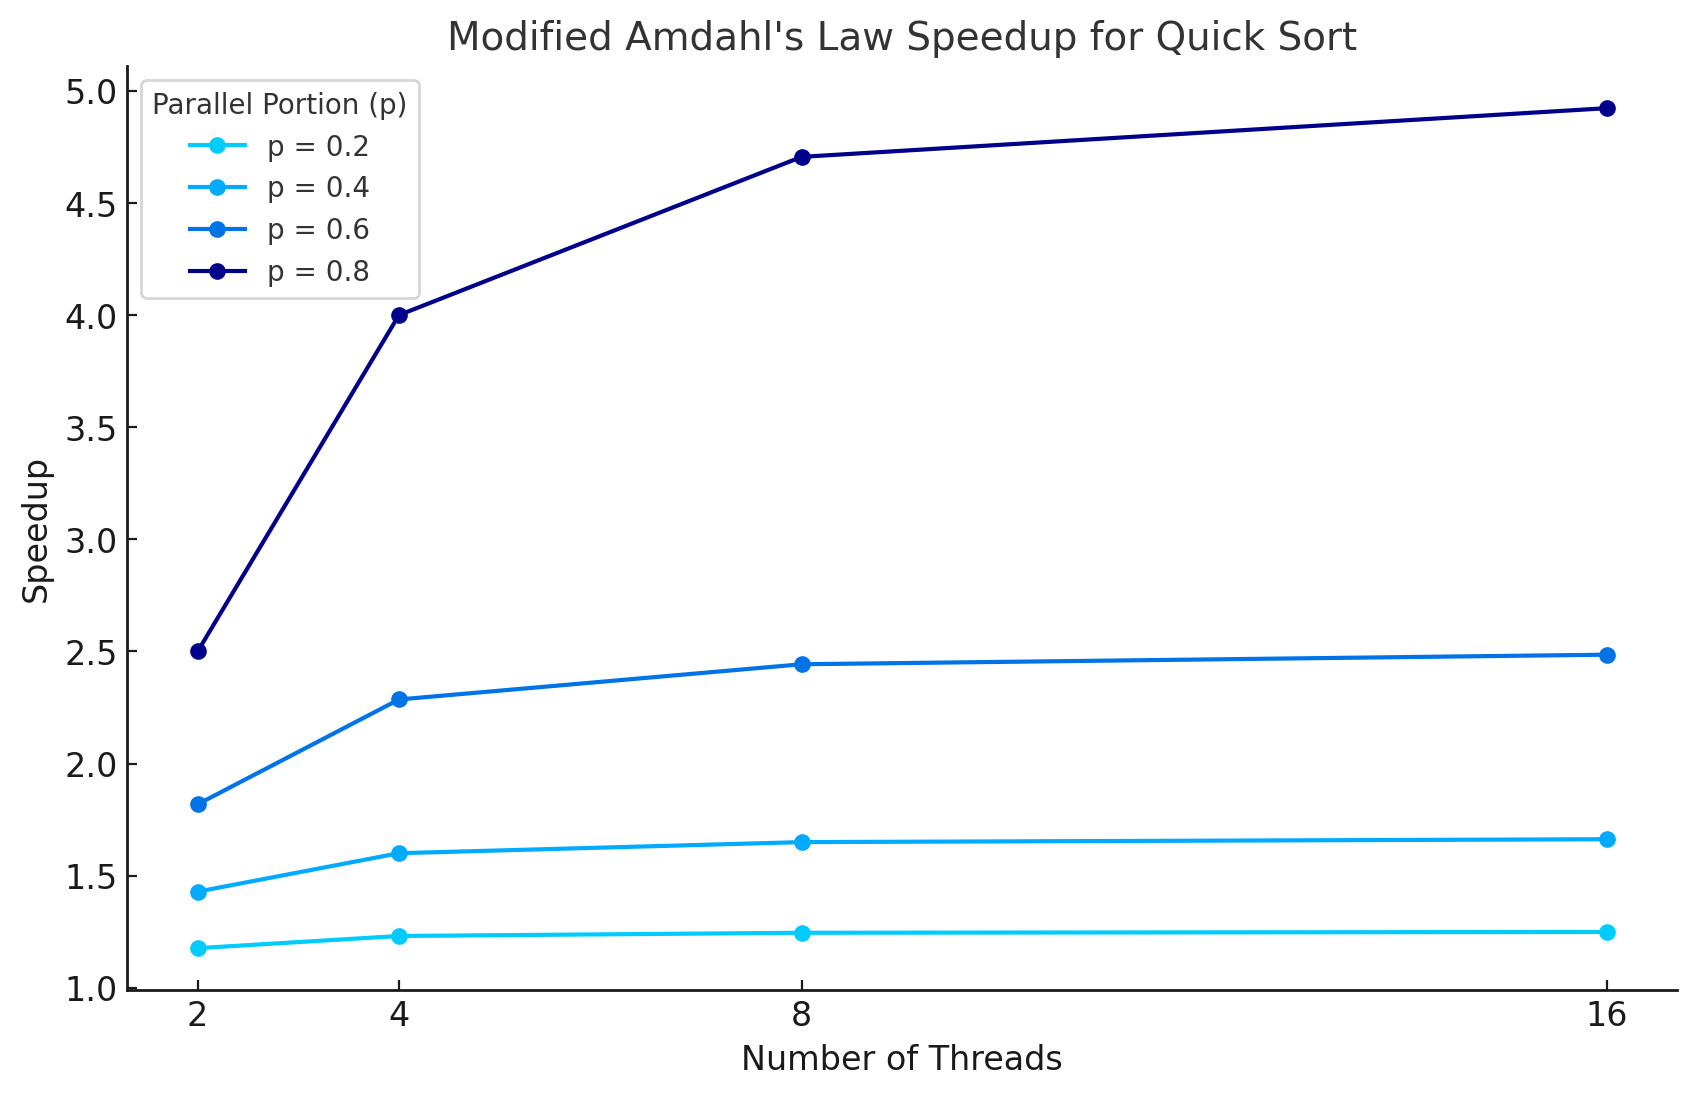
\includegraphics[width=1.0\linewidth]{LaTex/images/Amdahls Law.png}
    \caption{Speedup of Quick Sort using Modified Amdahl’s Law for different values of \(p\) and thread counts.}
    \label{fig:amdahls-law-speedup}
\end{figure}





\newpage
\section{ExecutorService Parallel Sort}

\subsection{Program Explanation}
\textbf{Source files:}

- `ExecutorServiceSort.java`

\subsubsection{Explanation}
In this task, we implemented a parallel quicksort using Java’s \texttt{ExecutorService} with a fixed thread pool. The algorithm recursively divides the array into subarrays, and tasks are submitted to the thread pool to sort each subarray concurrently. For smaller subarrays (size below 1000), sequential quicksort is used to minimize overhead. The \texttt{Future} objects synchronize the tasks, ensuring that both halves are fully sorted before proceeding. After sorting, the executor service is properly shut down to terminate all threads gracefully.

\subsubsection{Discussion}
The \texttt{ExecutorService} efficiently parallelizes quicksort by dividing the workload among multiple threads. This approach improves performance for larger arrays by reducing overall sorting time. However, managing threads and synchronizing tasks introduces some overhead, especially for smaller arrays where the cost of parallelism outweighs its benefits. Despite this, for larger arrays, the ExecutorService approach effectively distributes the sorting process and results in significant speedup.



\newpage
\section{ForkJoinPool and RecursiveAction}

\subsection{Program Explanation}
\textbf{Source files:}

- `ForkJoinSort.java`

\subsubsection{Explanation}
In this task, we implemented a parallel quicksort using Java's \texttt{ForkJoinPool} and \texttt{RecursiveAction}. The sorting process is split into smaller tasks using the \texttt{Worker} class, which extends \texttt{RecursiveAction}. If the subarray size exceeds a threshold (1000), the array is partitioned and two new tasks are created to sort the left and right subarrays concurrently. The \texttt{invokeAll()} method is used to execute the tasks in parallel. If the subarray is small enough, sequential quicksort is used to avoid the overhead of task creation.

\subsubsection{Discussion}
The \texttt{ForkJoinPool} efficiently parallelizes the sorting process by leveraging task decomposition, making it well-suited for larger arrays. The use of \texttt{RecursiveAction} allows for a clear division of labor between tasks, ensuring concurrent sorting of subarrays. However, for smaller arrays, the overhead of task creation and management can outweigh the benefits of parallelism. Overall, the ForkJoinPool approach improves performance by utilizing multiple threads, but the effectiveness depends on the array size and the chosen threshold.


\newpage
\section{ParallelStream and Lambda Functions}

\subsection{Program Explanation}
\textbf{Source files:}

- `ParallelStreamSort.java`

\subsubsection{Explanation}
In this task, we implemented a parallel quicksort using Java's \texttt{ParallelStream} and Lambda functions. The sorting algorithm partitions the array and then uses \texttt{Arrays.stream()} with \texttt{parallel()} to execute the sorting of subarrays concurrently. If a subarray is smaller than a threshold (1000), sequential quicksort is used. To control the number of threads, we wrap the parallel stream in a \texttt{ForkJoinPool}, which limits the number of threads to the specified amount. The pool ensures proper management of parallel tasks and is shut down after the sort completes.

\subsubsection{Discussion}
The use of \texttt{ParallelStream} and Lambda functions allows for a clean and functional approach to parallel sorting. It efficiently parallelizes the sorting process, especially for larger arrays. However, there is some overhead due to stream management, and for smaller arrays, the performance benefits diminish compared to a fully sequential approach. Overall, this method is effective in utilizing multiple cores and threads for large datasets, but the choice of threshold and thread management is crucial for optimal performance.


\newpage
\section{Performance Measurements with PDC}

\subsection{Instrumentation}
To measure performance, we instrumented each sorting algorithm to record execution time using \texttt{System.nanoTime()}. The tests were conducted with 1,000,000 elements, using thread counts of 2, 4, 8, 16, 32, 48, 64, and 96. For parallel algorithms, we ensured the thread pool and parallel streams were configured to match the specified thread count. Each algorithm was warmed up with 10 rounds before conducting 100 measurement rounds. The sequential implementation served as the baseline, while the JavaSort library was used as a reference for comparison.

\subsection{Execution Time and Speedup Plot}
The following graph presents the execution time for each sorting algorithm across varying thread counts. The speedup is normalized to the sequential sort. 

\begin{figure}[H]
    \centering
    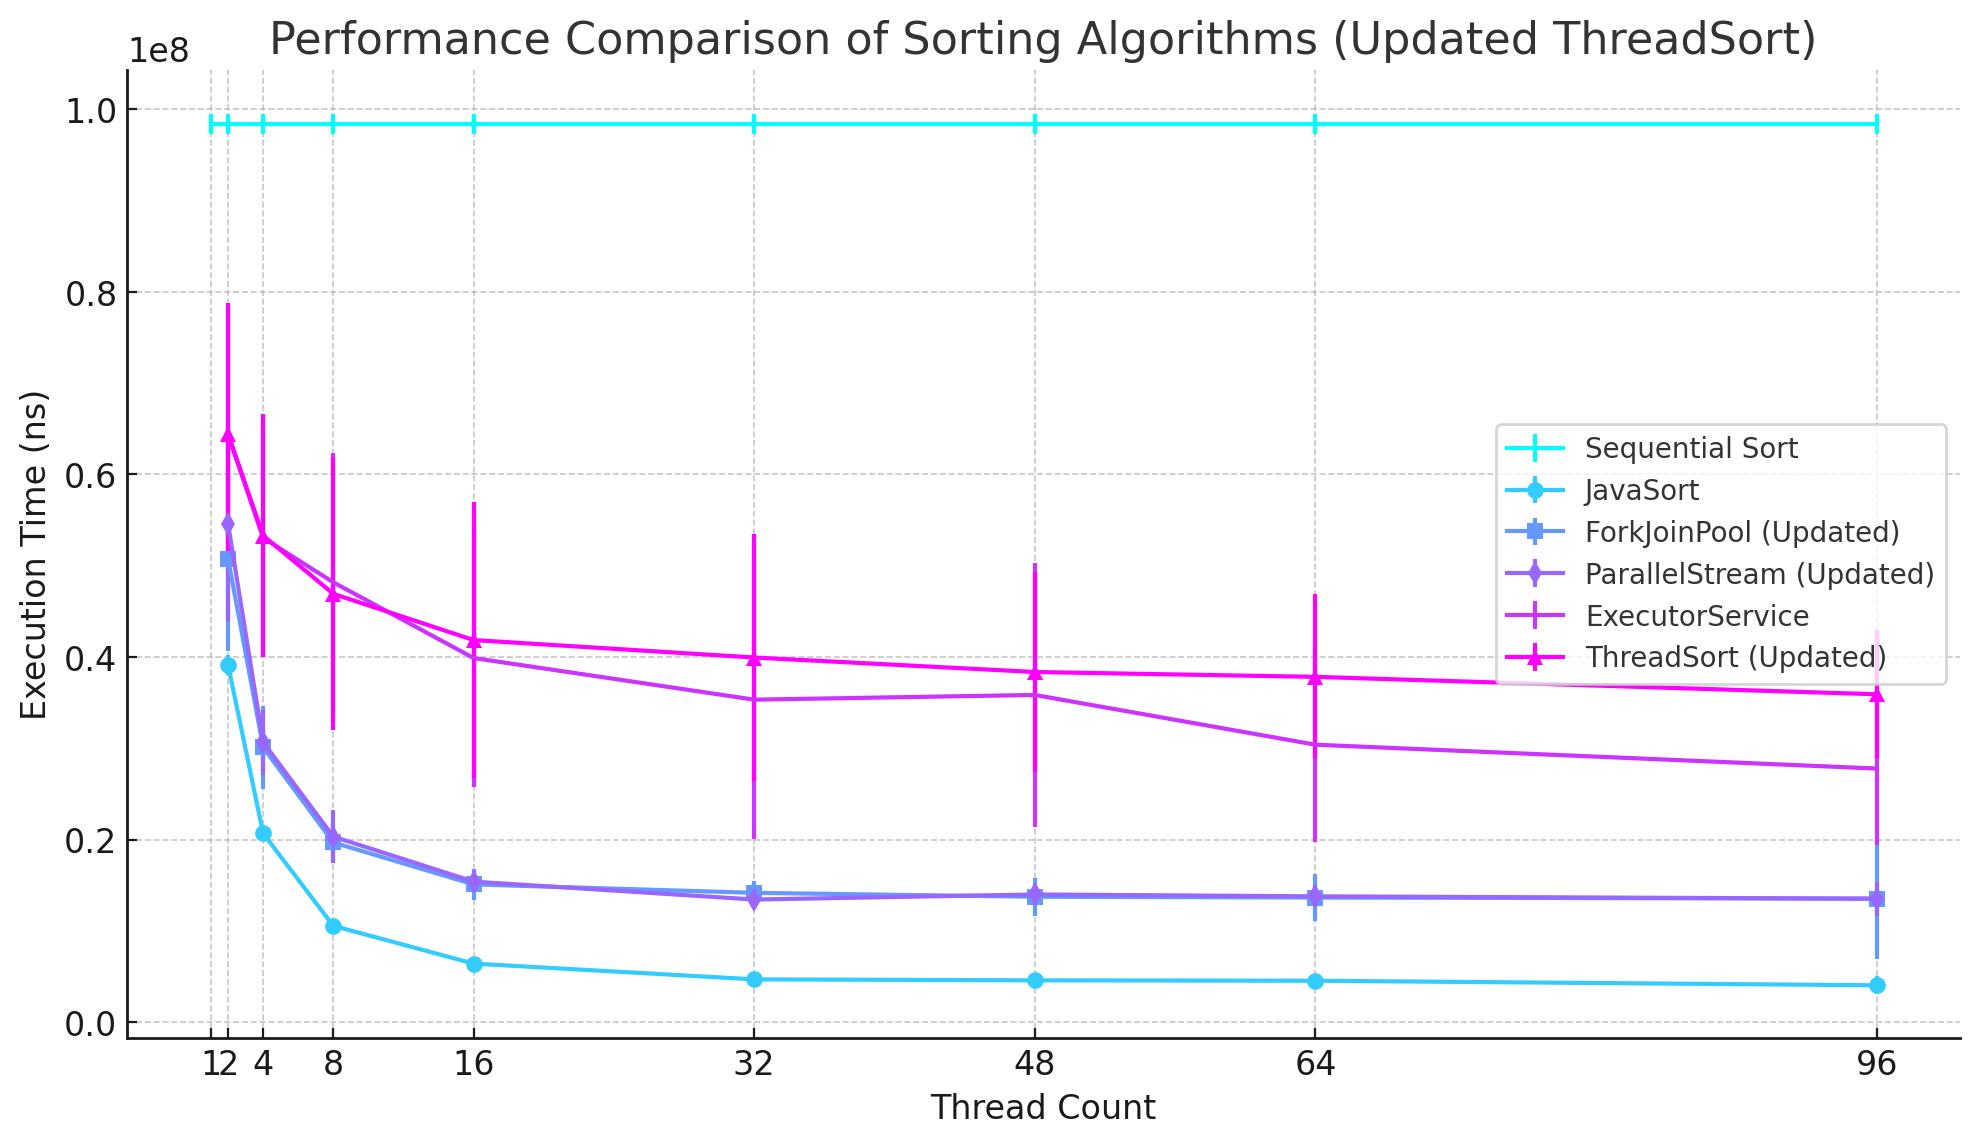
\includegraphics[width=1.0\linewidth]{LaTex/images/Lab2.png}
    \caption{Performance Comparison of Sorting Algorithms with Different Thread Counts.}
    \label{fig:sorting-performance}
\end{figure}

\subsubsection{Discussion}
As we expected, parallelized algorithms showed significant speedups compared to the sequential version, especially with larger thread counts. JavaSort exhibited the best overall performance, benefiting from optimized internal algorithms. ForkJoinPool and ExecutorService also performed well, but speedups plateaued after 32 threads due to thread management overhead. ParallelStream, though easy to implement, had higher overhead and showed diminishing returns earlier than ForkJoinPool or ExecutorService. The sequential algorithm remained consistent but was significantly outperformed by all parallel versions at higher thread counts.


\newpage
\section{ThreadSort using start() and join()}

\subsection{Program Explanation}
\textbf{Source files:}

- `ThreadSort.java`

\subsubsection{Explanation}
We did this extra task after realizing we had used PDC wrong during the presentation. For the task, we implemented a parallel quicksort using Java's native \texttt{Thread} class with the \texttt{start()} and \texttt{join()} methods. The array is divided into chunks, each of which is assigned to a separate thread for sorting. The number of threads used is specified by the \texttt{threads} parameter. Each thread sorts its designated chunk using a sequential quicksort method. 

\subsubsection{Discussion}
The use of Java's \texttt{Thread} class allows direct control over thread management but also introduces challenges in managing thread creation and synchronization. This implementation effectively parallelizes sorting for medium to large arrays, where each thread can handle a significant chunk of data. Additionally, for smaller arrays or when the chunk size is below the threshold, the overhead from thread management can lead to longer execution times compared to other parallel methods like \texttt{ForkJoinPool}. Despite these limitations, the implementation demonstrates the basics of parallelism using Java threads.


\newpage
\printbibliography

\end{document}
